%%%%%%%%%%%%%%%%%%%%%%%%%%%%%%%%%%%%%
%                                   %
% Compile with XeLaTeX and biber    %
%                                   %
% Questions or comments:            %
%                                   %
% joshua dot mcneill at uga dot edu %
%                                   %
%%%%%%%%%%%%%%%%%%%%%%%%%%%%%%%%%%%%%

\documentclass{beamer}
  % Read in standard preamble (cosmetic stuff)
  %%%%%%%%%%%%%%%%%%%%%%%%%%%%%%%%%%%%%%%%%%%%%%%%%%%%%%%%%%%%%%%%
% This is a standard preamble used in for all slide documents. %
% It basically contains cosmetic settings.                     %
%                                                              %
% Joshua McNeill                                               %
% joshua dot mcneill at uga dot edu                            %
%%%%%%%%%%%%%%%%%%%%%%%%%%%%%%%%%%%%%%%%%%%%%%%%%%%%%%%%%%%%%%%%

% Beamer settings
% \usetheme{Berkeley}
\usetheme{CambridgeUS}
% \usecolortheme{dove}
% \usecolortheme{rose}
\usecolortheme{seagull}
\usefonttheme{professionalfonts}
\usefonttheme{serif}
\setbeamertemplate{bibliography item}{}

% Packages and settings
\usepackage{fontspec}
  \setmainfont{Charis SIL}
\usepackage{hyperref}
  \hypersetup{colorlinks=true,
              allcolors=blue}
\usepackage{graphicx}
  \graphicspath{{../../figures/}}
\usepackage[normalem]{ulem}
\usepackage{enumerate}

% Document information
\author{M. McNeill}
\title[FREN2001]{Français 2001}
\institute{\url{joshua.mcneill@uga.edu}}
\date{}

%% Custom commands
% Lexical items
\newcommand{\lexi}[1]{\textit{#1}}
% Gloss
\newcommand{\gloss}[1]{`#1'}
\newcommand{\tinygloss}[1]{{\tiny`#1'}}
% Orthographic representations
\newcommand{\orth}[1]{$\langle$#1$\rangle$}
% Utterances (pragmatics)
\newcommand{\uttr}[1]{`#1'}
% Sentences (pragmatics)
\newcommand{\sent}[1]{\textit{#1}}
% Base dir for definitions
\newcommand{\defs}{../definitions}


  % Packages and settings

  % Document information
  \subtitle[Femmes et questions]{Les femmes et les questions}

\begin{document}
  % Read in the standard intro slides (title page and table of contents)
  \begin{frame}
    \titlepage
    \tiny{Office: % Basically a variable for office hours location
Gilbert 121\\
          Office hours: % Basically a variable for office hours
 lundi, mercredi, vendredi 10:10--11:10
}
  \end{frame}

  \begin{frame}{Annonces}
    \begin{itemize}
      \item
      \item[] \gloss{}
    \end{itemize}
  \end{frame}

  \begin{frame}{Des femmes connues}
    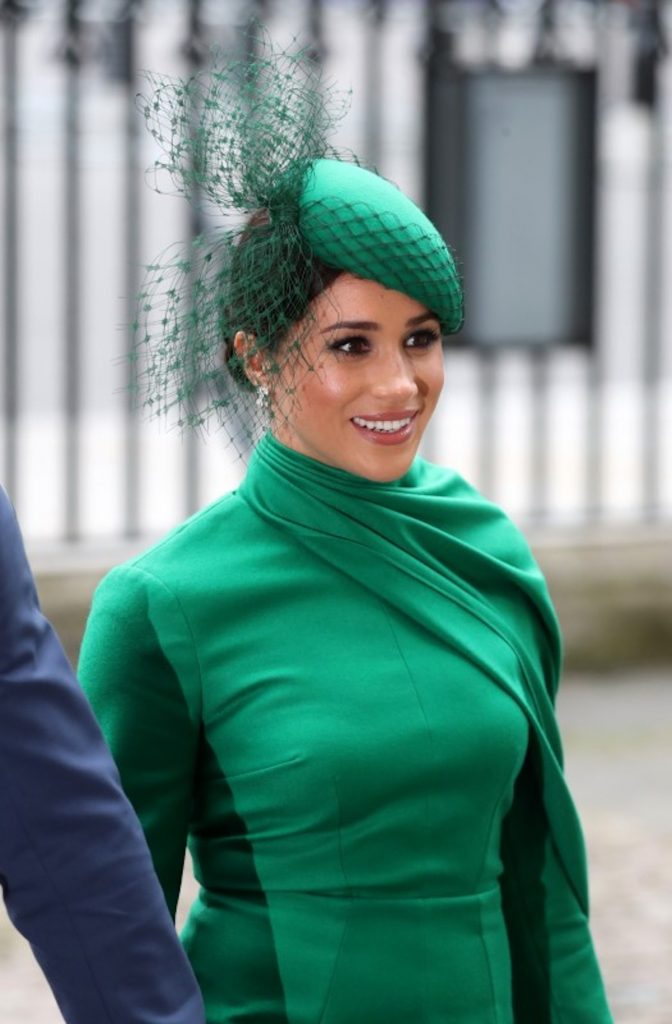
\includegraphics[scale=0.5]{meghan_markle.jpg}
  \end{frame}

  \begin{frame}{Des femmes connues}
    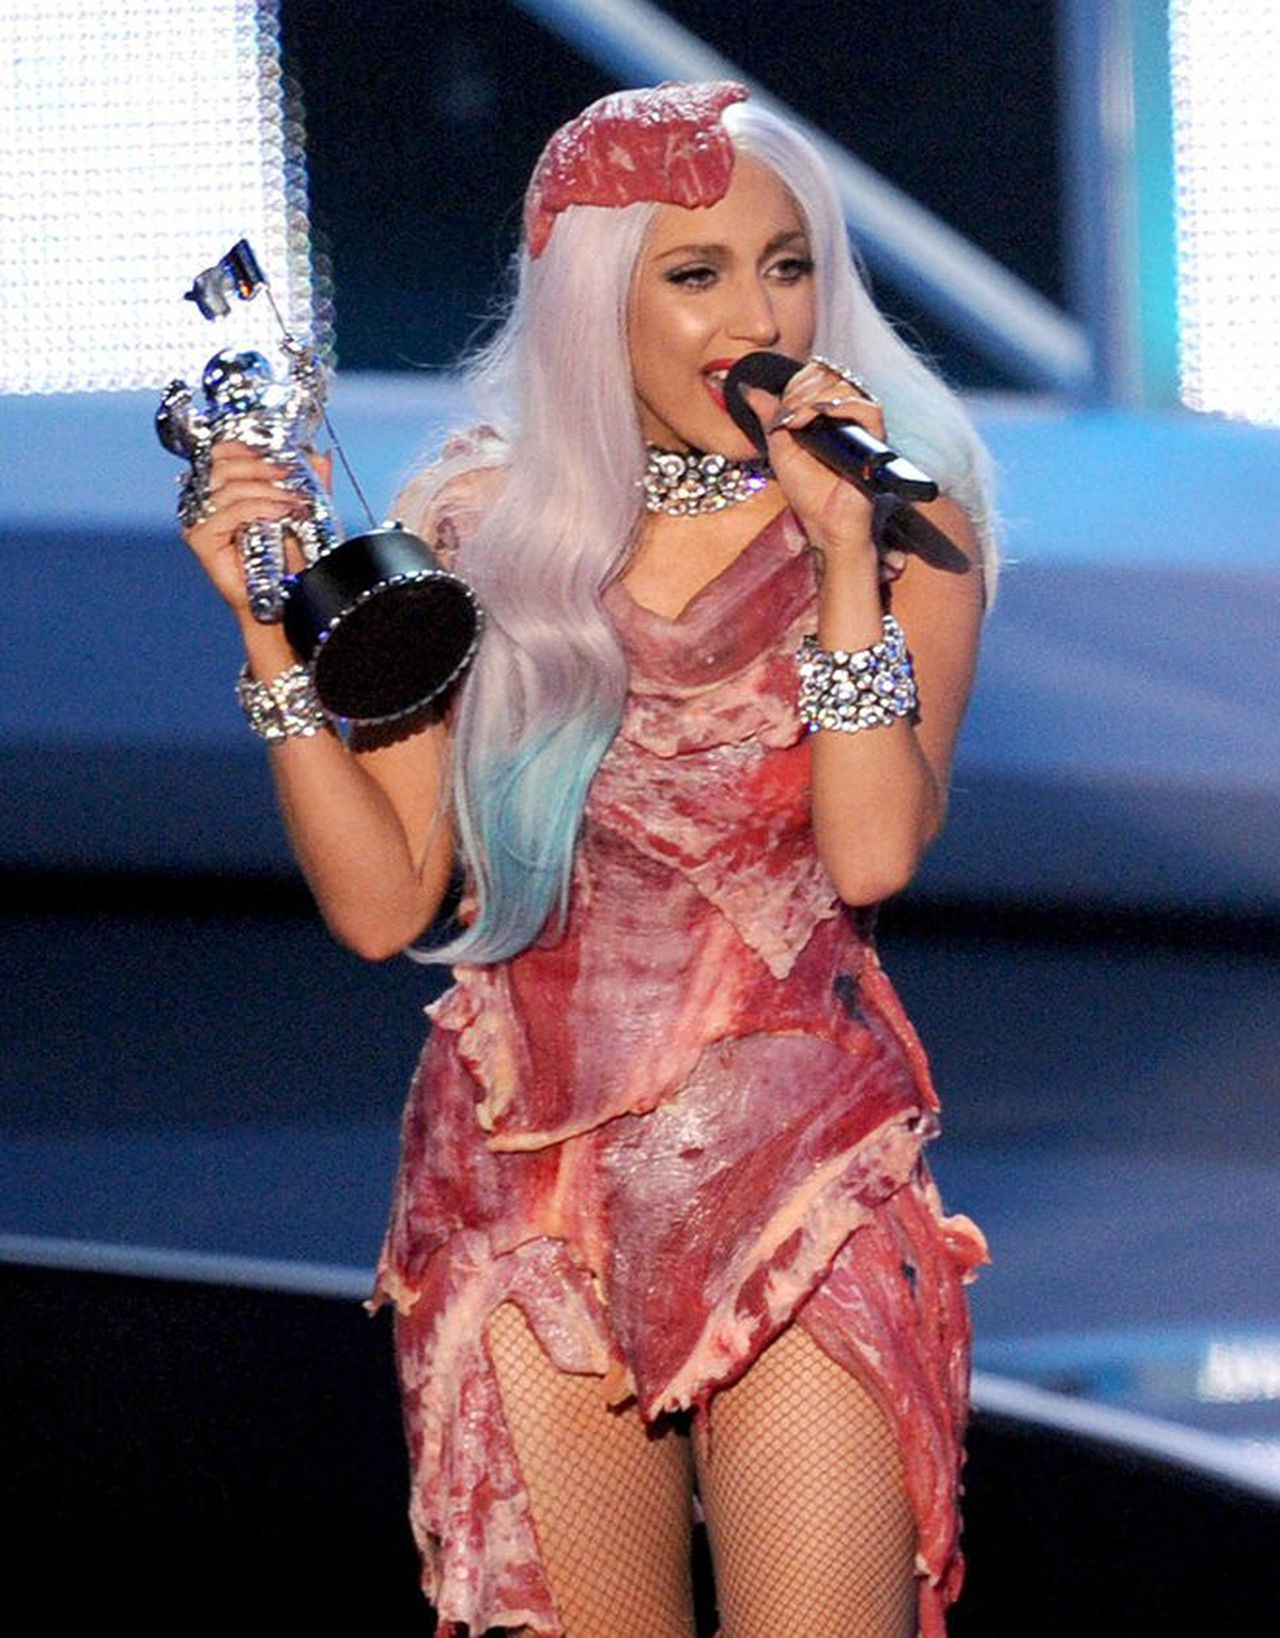
\includegraphics[scale=0.5]{lady_gaga.jpg}
  \end{frame}

  \begin{frame}{Des femmes connues}
    
\includegraphics[scale=0.5]{oprah.jpg}
  \end{frame}

  \begin{frame}{Des femmes connues}
    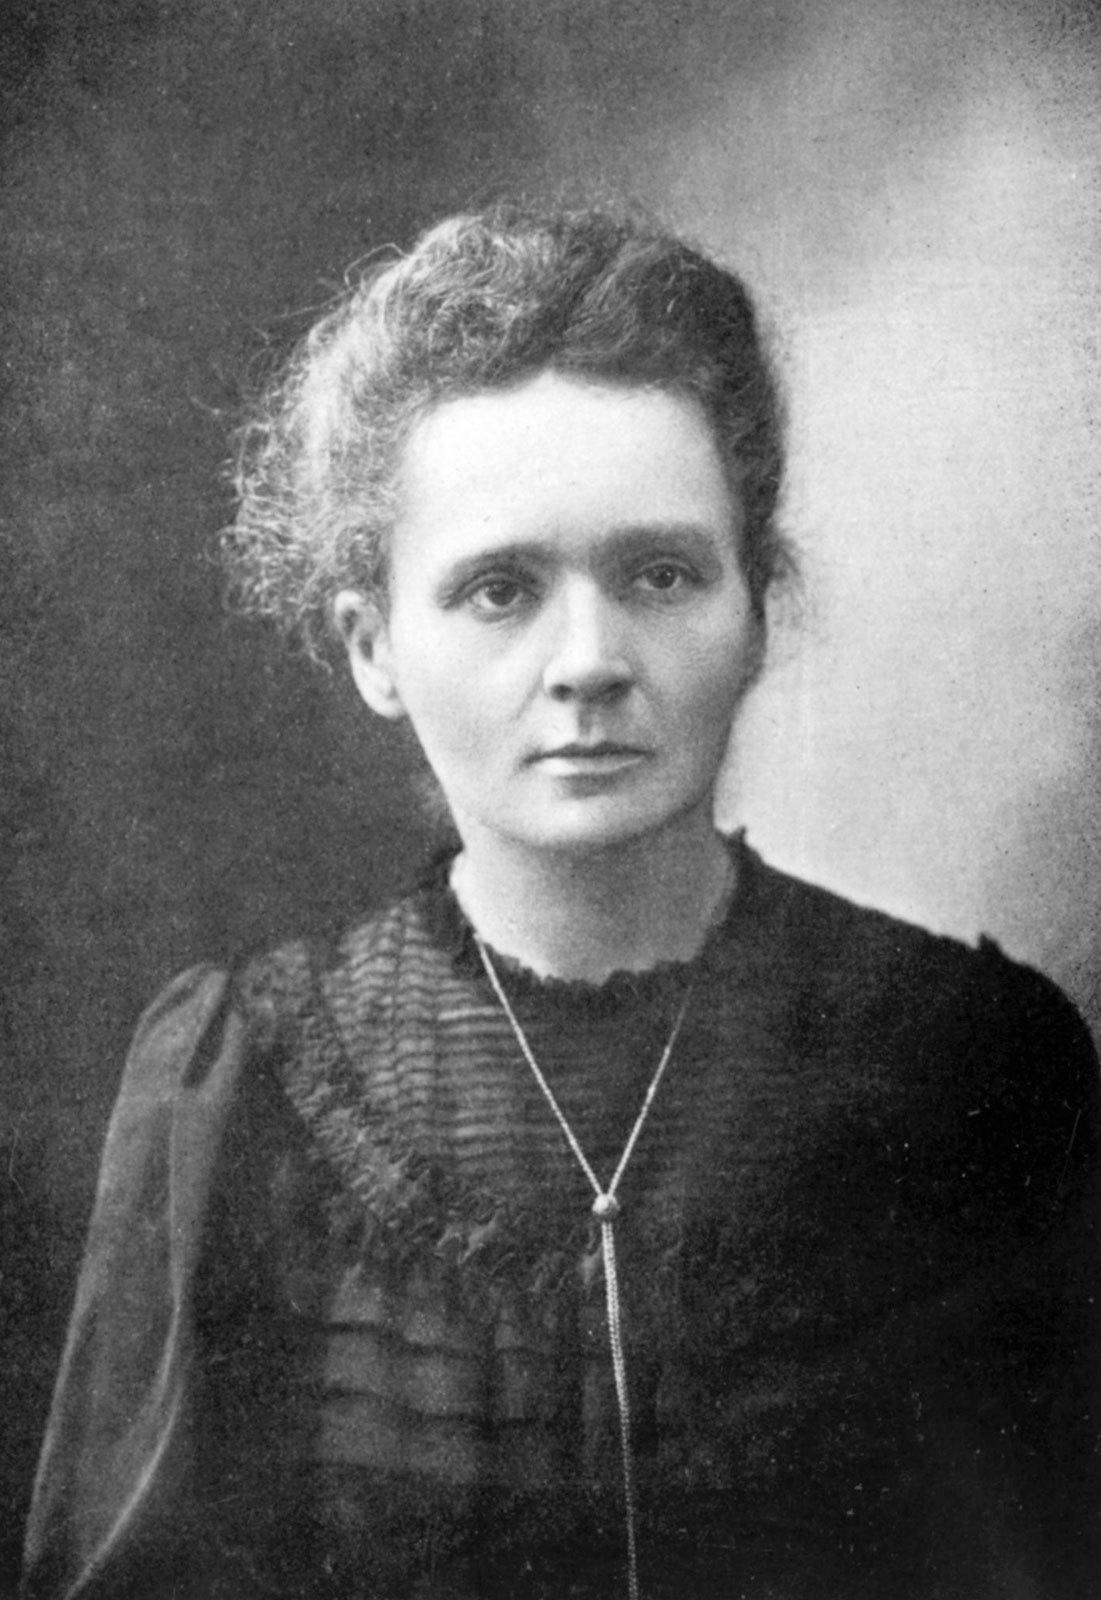
\includegraphics[scale=0.5]{marie_curie.jpg}
  \end{frame}

  \begin{frame}{Des femmes connues}
    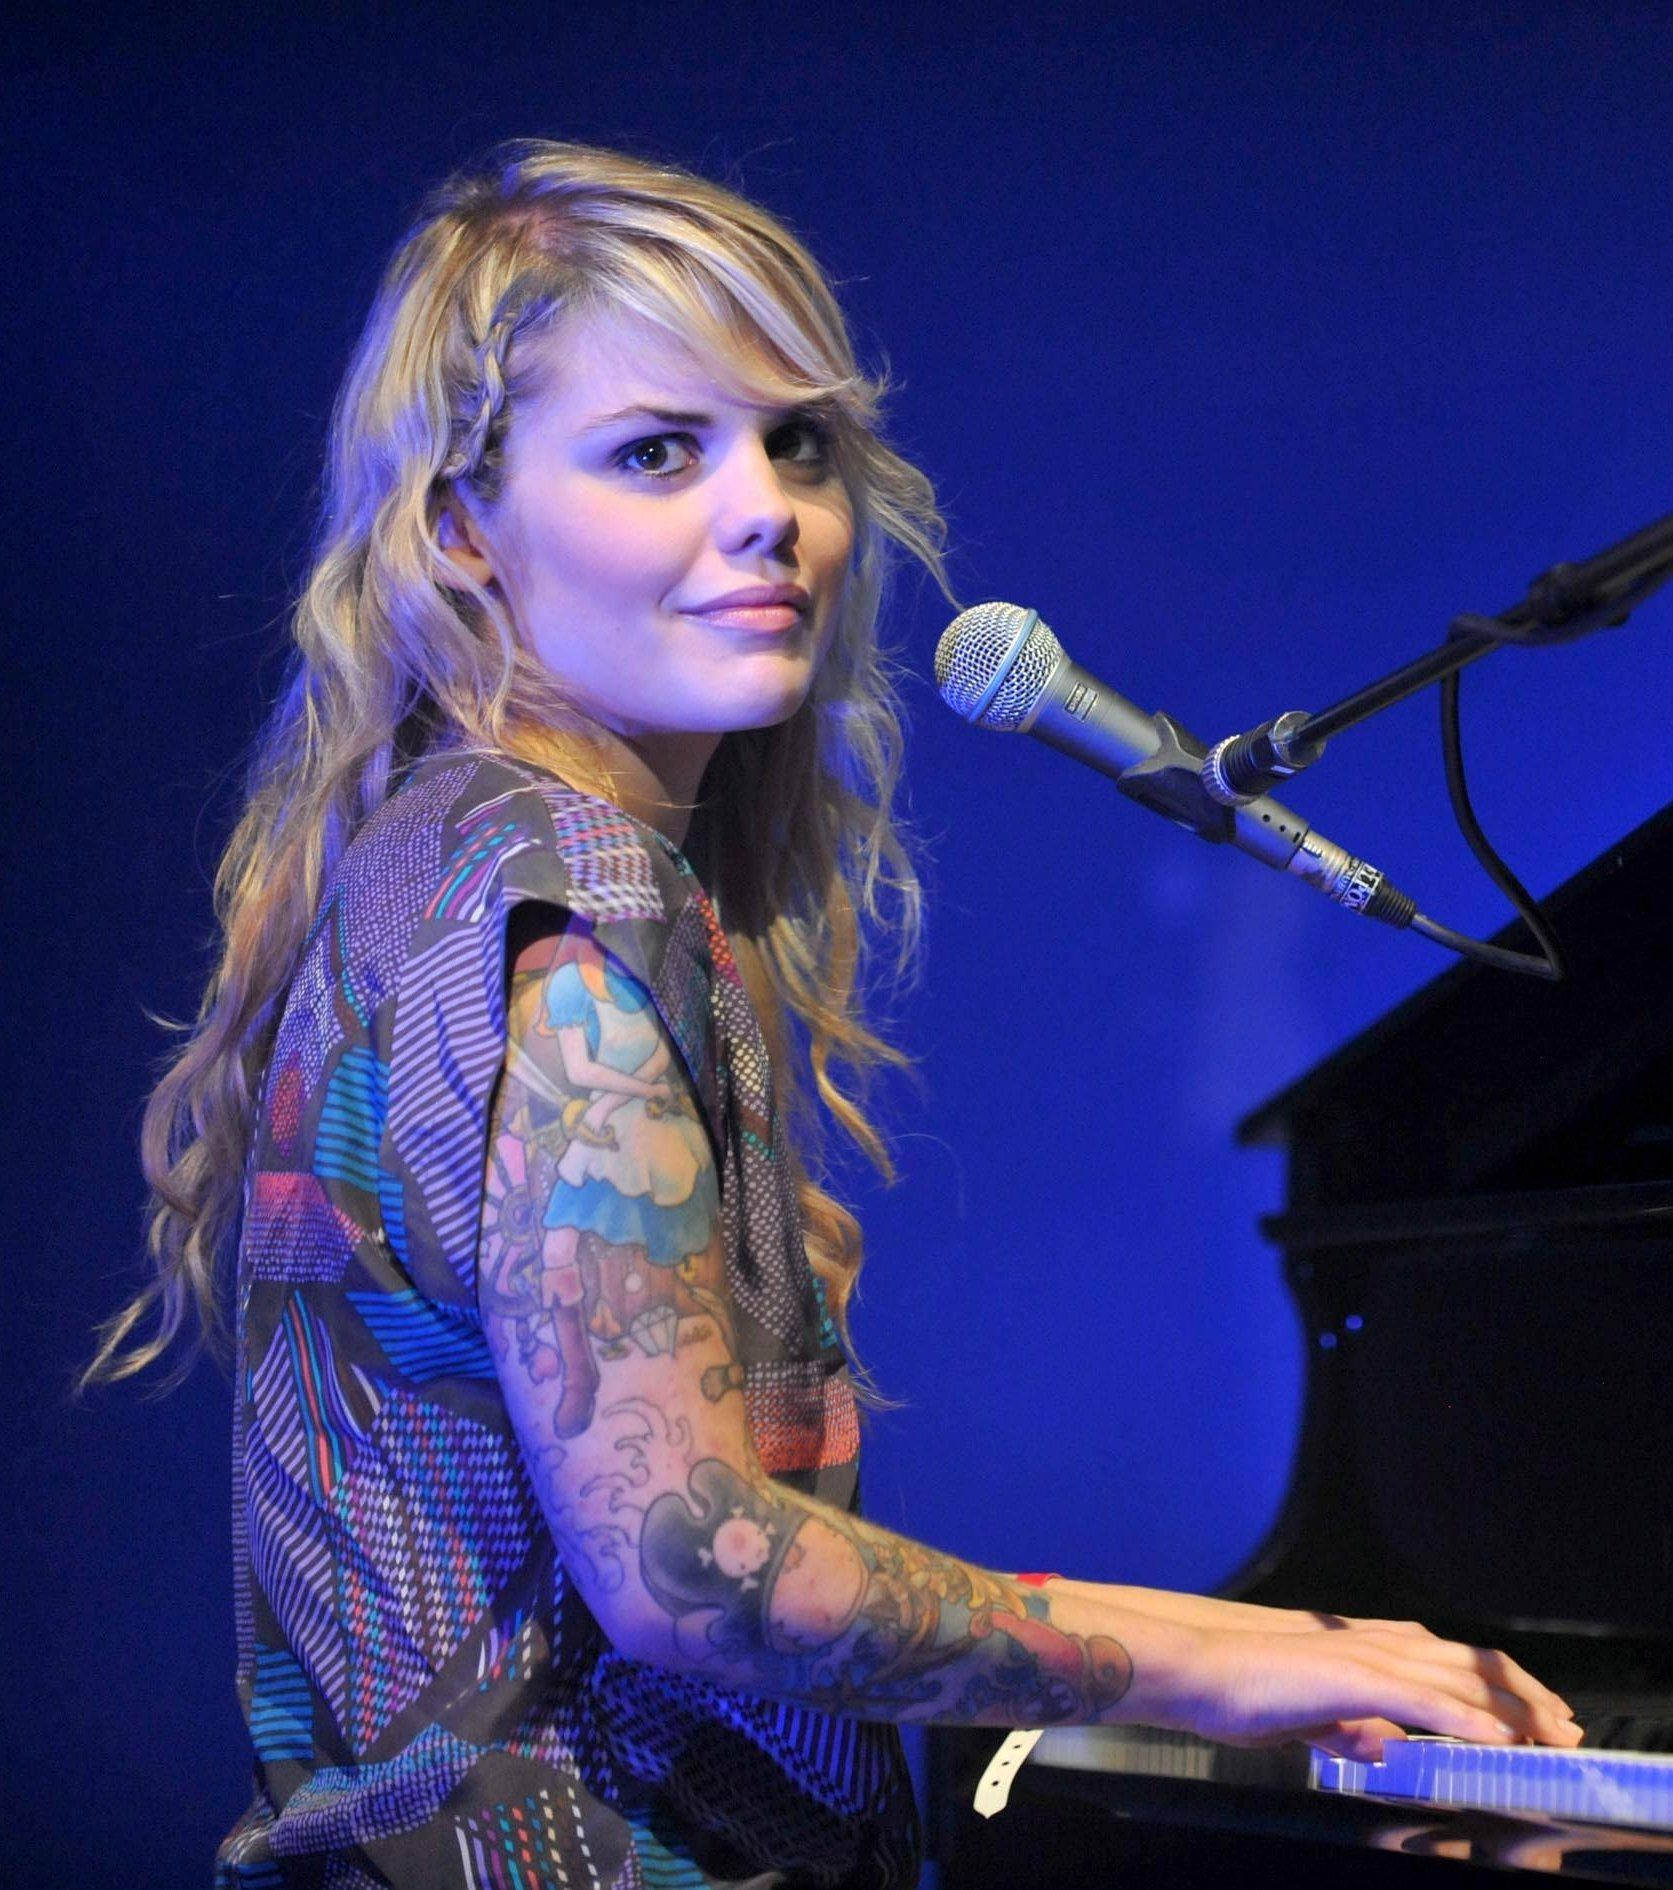
\includegraphics[scale=0.5]{coeur_de_pirate.jpg}
  \end{frame}

  \begin{frame}{}
    \begin{center}
      \Large Quiz
    \end{center}
  \end{frame}

  \begin{frame}{Une personne connue}
    En groupes de 3 ou 4, décrivez des femmes connues chacun à son tour, et faites deviner leurs identités à vos camarades. Décrivez non seulement leurs traits physiques mais leurs personnalités et activités. \\
    \tinygloss{In groups of 3 or 4, take turns describing well-known women, and have your groupmates guess at her identity.
    Describe not just their physical features but their personalities and activities.}
  \end{frame}


  \begin{frame}{}
    % As a class, show some statements about someone and have the class name some questions that you might ask to get more information.
  \end{frame}

  \begin{frame}{Entrevue}
    Avec un partenaire, faites des entrevues en posant des questions aux sujets suivants.  \\
    \tinygloss{With a partner, interview each other by asking questions about the following subjects.}
    \begin{enumerate}
      \item les amis
      \item la musique
      \item le sport
      \item les animaux
    \end{enumerate}
  \end{frame}

  \begin{frame}{}
    \begin{center}
      \Large Questions?
    \end{center}
  \end{frame}
\end{document}
